\section{Software}

\subsection{Smartphone-App: Java}
\label{sec:smartphoneapp}

Um die autonome Laufkatze zu starten wird eine Smartphone-App verwendet. Dazu muss sich das Smartphone im selben Netzwerk wie der Raspi befinden. Der Raspi übernimmt dabei die Rolle des Servers, und das Smartphone verbindet sich als Client mit ihm. Betätigt der Anwender die Starttaste der App, verbindet sich das Smartphone mit dem Raspi, und die Laufkatze wird gestartet. Sobald die Last aufgenommen wurde, sendet der Raspi fortlaufend die aktuellen Koordinaten der Last an die Smartphone-App. Auf diese Weise sieht der Anwender ununterbrochen die aktuellen Lastkoordinaten auf seinem Smartphone. Dabei zeigt das Smartphone lediglich die empfangenen Koordinaten an und übernimmt keinerlei Logik.

Damit die Kommunikation zwischen Smartphone und Raspi funktioniert, müssen sich beide Geräte im selben Netzwerk befinden. Dazu wird mittels eines \textit{maplite}-Routers ein eigenes Netzwerk mit der SSID \texttt{pren7} aufgebaut. Mit diesem Netzwerk verbinden sich der Raspi und das Smartphone. Damit sich das Smartphone mit dem Raspi verbinden kann, wurde für den Raspi eine statische IP-Adresse konfiguriert.

Für die Entwicklung der Smartphone-App wurde das Android Studio verwendet. Das Android Studio bietet viele Vorteile für die Entwicklung, zum Beispiel einen integrierten Emulator, oder das Debuggen direkt auf dem Smartphone.

\imgrefplain{fig:smartphoneapp} zeigt die Benutzeroberfläche der Smartphone-App.

\begin{figure}[H]
    \centering
    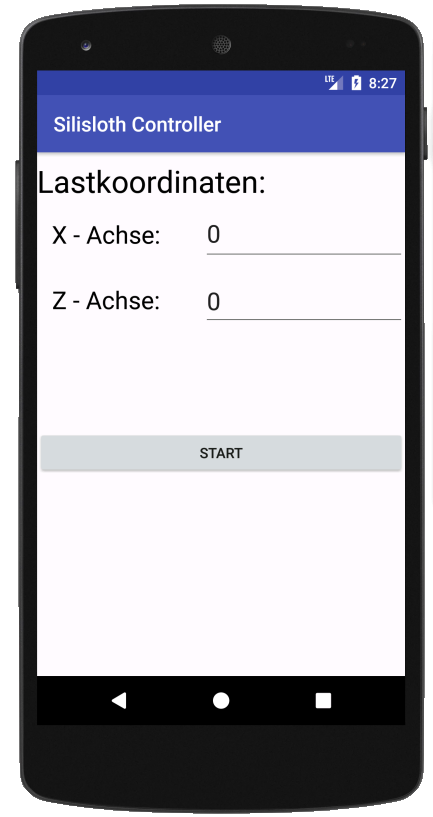
\includegraphics[width=0.25\linewidth]{pics/smartphoneapp.png}
    \caption{Die Smartphone-App zur Steuerung von \textit{Silisloth} und zum Ablesen der Koordinaten}
    \label{fig:smartphoneapp}
\end{figure}

\subsection{Raspi: Python}
\label{sec:raspi}

Die übergeordnete Steuerung und Koordination von \textit{Silisloth} wurde auf dem Raspi mit Python umgesetzt. Der Quellcode zum Projekt findet sich im Anhang (\texttt{silisloth-raspi.zip})

\begin{figure}
    \centering
    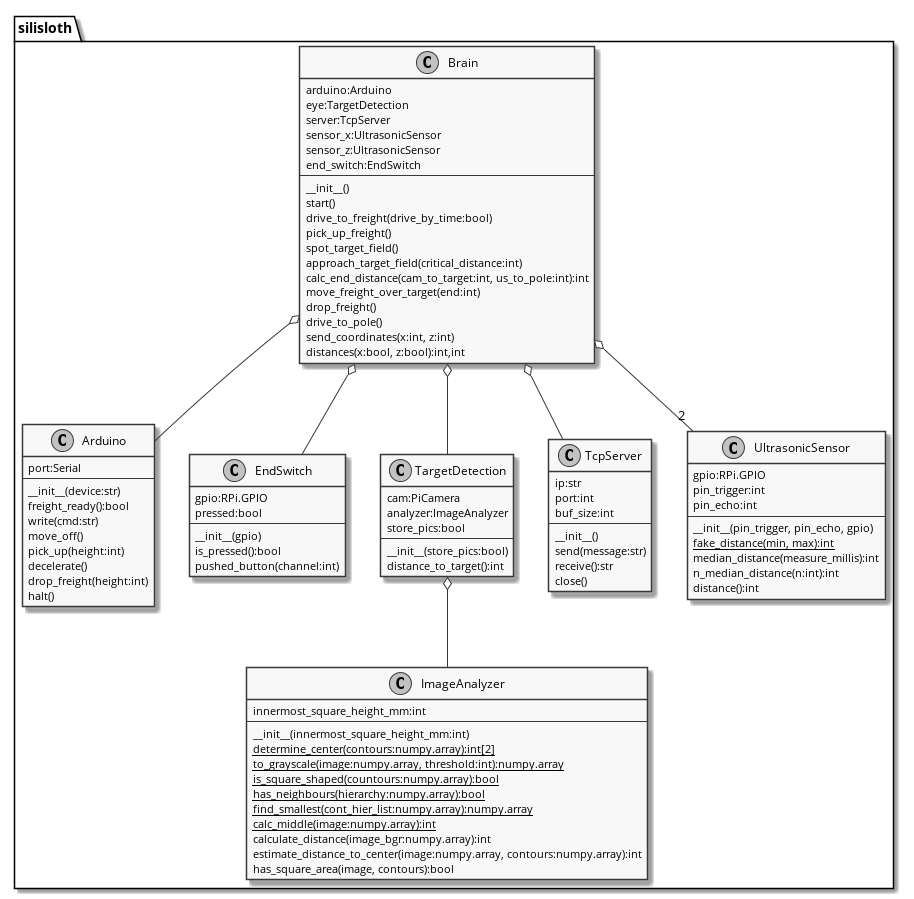
\includegraphics[width=\textwidth]{graphs/klassendiagramm.png}
    \caption{Das Klassendiagramm des Python-Projektes}
    \label{fig:klassendiagramm}
\end{figure}

\subsubsection{Projektstruktur}

Das Projekt besteht aus verschiedenen Quellcodedateien:

\begin{description}
    \item[\texttt{Arduino.py}] Kommunikation mit dem Arduino per serieller Schnittstelle (USB): Die angebotenen Funktionen bieten eine selbsterklärende Schnittstelle für die zu erteilenden und empfangenden Befehle.
    \item[\texttt{Brain.py}] Die übergeordnete Programmlogik: Der ganze Ablauf (\secref{sec:ablauf}) wird von diesem Skript gesteuert.
    \item[\texttt{EndSwitch.py}] Ansteuerung des Mikroendschalters: Es wird eine Funktion zur Verfügung gestellt, die blockierend auf das Betätigen des Mikroendschalters wartet.
    \item[\texttt{ImageAnalyzer.py}] Die Bildverarbeitungslogik: Verarbeitet ein einzelnes Bild und gibt eine Millimeterangabe zurück, die den optischen Abstand in x-Richtung von Kameralinse zum Zielfeldmittelpunkt in Millimetern zurückgibt.
    \item[\texttt{Log.py}] Logger-Konfiguration und -Format für sämtliche im Projekt geschriebenen Logmeldungen: Für die Ausgabe auf den Bildschirm wird aus Gründen der Übersichtlichkeit ein tieferes Log-Level verwendet als für die Ausgabe in die Logdatei.
    \item[\texttt{TargetDetection.py}] Fassade für den \texttt{ImageAnalyzer}: Kümmert sich um die Aufnahme von Bildern und stellt eine vereinfachte Schnittstelle für die Bildverarbeitungslogik und das Abspeichern der aufgenommenen Bildern zu Debug-Zwecken zur Verfügung.
    \item[\texttt{TcpServer.py}] Kommunikation zum Smartphone: Wartet blockierend auf eine eingehende Verbindung und schickt die formatierte Zeichenkette mit den Koordinaten an die Smartphone-App.
    \item[\texttt{UltrasonicSensor.py}] Ansteuerung der Ultraschallsensoren: Bietet Funktionen zur Erstellung von Messreihen. Es kann eine bestimmte Anzahl von Messungen erstellt oder eine bestimmte Zeit lang gemessen werden. Von der Messreihe wird der Median-Wert zurückgegeben, was die Messung robust für Fehlmessungen macht \cite[S. 46-48]{pren1}.
\end{description}

Zum Testen einzelner Komponenten wurden folgende Demo-Programme entwickelt:

\begin{description}
    \item[\texttt{ArduinoMock.py}] Testprogramm für die serielle Kommunikation mit dem Arduino: Befehle können direkt über die Kommandozeile an den Arduino gesendet werden, was zum Testen und zur Fehlersuche hilfreich ist.
    \item[\texttt{ImageAnalyzerDemo.py}] Testprogramm für die Zielfelderkennung: Verarbeitet eine im Dateisystem abgespeicherte Bildserie und gibt die dabei errechneten Abstände vom Zielfeldmittelpunkt auf der Kommandozeile aus.
    \item[\texttt{TargetDetectionDemo.py}] Weiteres Testprogramm für die Zielfelderkennung: Im Gegensatz zur \texttt{ImageAnalyzerDemo} werden die zu verarbeiteten Bilder direkt über die Raspi-Kamera aufgenommen.
    \item[\texttt{UltrasonicDemo.py}] Testprogramm für die Ultraschallsensoren: Es wird eine bestimmte Anzahl von Messungen durchgeführt. Der Median des Messergebnis wird auf die Kommandozeile ausgegeben. Der Vorgang wird endlos wiederholt, womit die Messungen beim manuellen Fahren am Seil überprüft werden können.
\end{description}

\subsubsection{Eingesetzte Python-Bibliotheken}

\begin{description}
    \item[OpenCV] Bildverarbeitungsbibliothek mit Python-Interface \cite{opencv}
    \item[NumPy] Matrizenberechnungen: OpenCV verwendet Matrizen als Datenstruktur für die Bilder \cite{numpy}
    \item[RPi.GPIO] Ansteuerung von GPIO-Ports: Interaktion mit Ultraschallsensoren und dem Mikroendschalter \cite{rpigpio}
    \item[Picamera] Ansteuerung der Raspi-Kamera zur Aufnahme von Bildern \cite{picamera}
    \item[PySerial] Ansteuerung der seriellen Schnittstelle: Kommunikation per USB-Verbindung zum Arduino \cite{pyserial}
\end{description}

\subsection{Arduino: C}

\label{sec:arduino}

Die Motorensteuerung wurde auf dem Arduino umgesetzt. Der Quellcode zum Projekt findet sich im Anhang (\texttt{silisloth-arduino.zip}). Das Projekt ist in folgende Quellcodedateien aufgeteilt:

\begin{description}
    \item[\texttt{Sloth\_Main.ino}] Definition und Initialisierung von globalen Variablen und Tasks.
    \item[\texttt{Sloth\_Communication.ino}] Kommunikation mit dem Raspi per serieller Schnittstelle (\secref{sec:raspi-arduino})
    \item[\texttt{Sloth\_StateMachine.ino}] Die Programmlogik, gemäss einer State-Machine (\imgref{fig:arduino-statemachine})
    \item[\texttt{Sloth\_Functions.ino}] Implementierung diverser Funktionen
\end{description}

Es wurden folgende Arduino-Bibliotheken eingesetzt:

\begin{description}
    \item[Wire] Kommunikation mit I2C
    \item[FreeRTOS] Multitasking (Kommunikation und State-Machine)
    \item[Adafruid\_Motorshield] Ansteuerung von Motoren via Motor Shield
    \item[Utility] PWM

\end{description}

Die State-Machine (\imgref{fig:arduino-statemachine}) gibt Auskunft über die internen Stati und die Befehle, die intern für die Transitionen verwendet wurden.

\begin{figure}
    \centering
    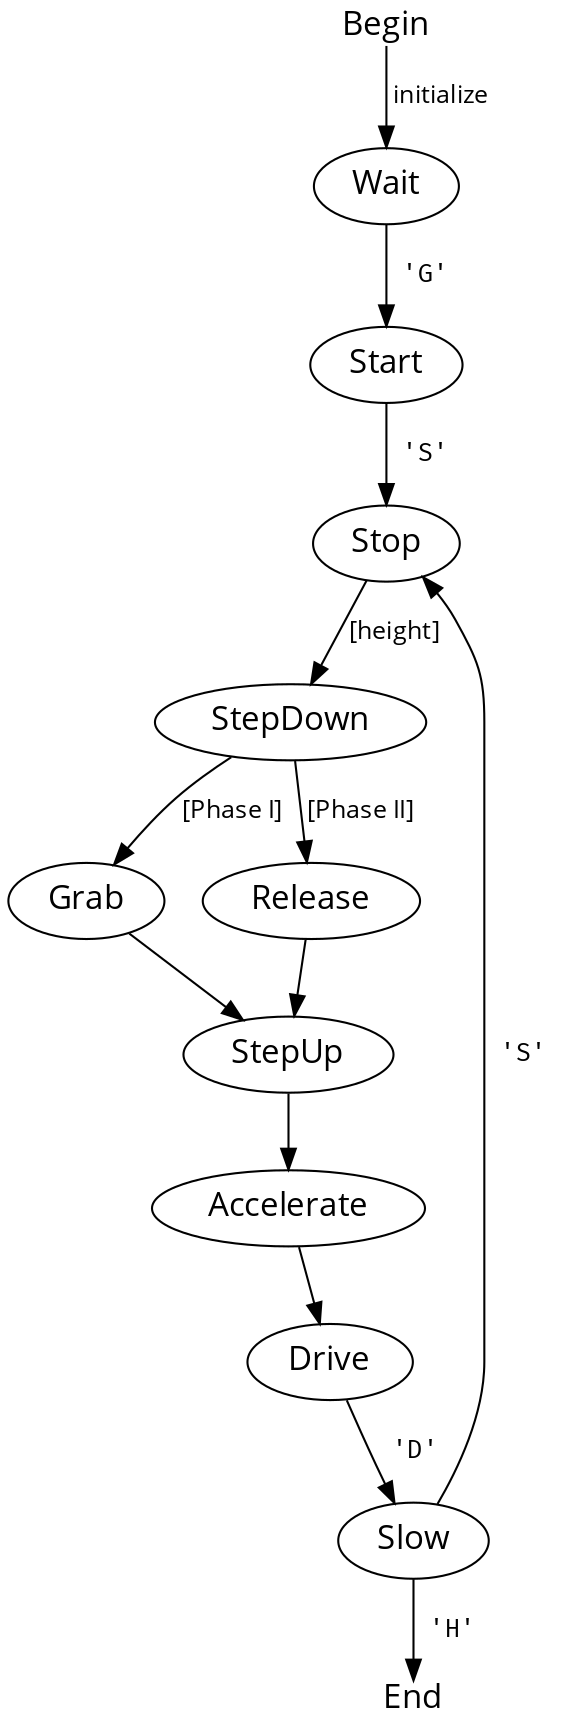
\includegraphics[height=\textheight]{graphs/arduino-statemachine.png}
    \caption{Die State-Machine der Arduino-Lösung}
    \label{fig:arduino-statemachine}
\end{figure}

